%                                                                 aa.dem
% AA vers. 9.1, LaTeX class for Astronomy & Astrophysics
% demonstration file
%                                                       (c) EDP Sciences
%-----------------------------------------------------------------------
%
%\documentclass[referee]{aa} % for a referee version
%\documentclass[onecolumn]{aa} % for a paper on 1 column  
%\documentclass[longauth]{aa} % for the long lists of affiliations 
%\documentclass[letter]{aa} % for the letters 
%\documentclass[bibyear]{aa} % if the references are not structured 
%                              according to the author-year natbib style


%
\documentclass{aa}  

%
\usepackage{graphicx}
\graphicspath{ {../figures/} }
%%%%%%%%%%%%%%%%%%%%%%%%%%%%%%%%%%%%%%%%
\usepackage{txfonts}
%%%%%%%%%%%%%%%%%%%%%%%%%%%%%%%%%%%%%%%%
\usepackage{amsmath}
\usepackage{subfigure}
\usepackage{booktabs}
\usepackage{hyperref}
%\usepackage[options]{hyperref}
% To add links in your PDF file, use the package "hyperref"
% with options according to your LaTeX or PDFLaTeX drivers.
%
\begin{document} 



   \title{Stellar parameters determination}

   
   \subtitle{Project I - Computational Astronomy}

   \author{Rui Peixoto}

   \institute{Departamento de Física e Astronomia, Faculdade de Ciências,
     Universidade do Porto}

%   \date{Received September 15, 1996; accepted March 16, 1997}

% \abstract{}{}{}{}{} 
% 5 {} token are mandatory
 
  \abstract
  % context heading (optional)
  % {} leave it empty if necessary  
   {}
  % aims heading (mandatory)
   {A systematic and efficient method to determine stellar parameters from observed spectra by
     comparison with synthetic spectra is developed and implemented.}
  % methods heading (mandatory)
   {Stellar parameters are estimated and observed spectra are compared with
     preselected synthetic spectra by equivalent width comparison of select fitted
     lines. Selected synthetic spectra are then processed and
     interpolated to facilitate comparison with observed spectra.}
  % results heading (mandatory)
   {Computational method is implemented and two stars analysed. Sensibility to a
     stars' high rotational velocity, effects of experimental noise, good fit
     conditions are discussed and pathological cases analysed.}
  % conclusions heading (optional), leave it empty if necessary 
   {}

%   \keywords{giant planet formation --
%                $\kappa$-mechanism --
%                stability of gas spheres
%               }

   \maketitle
%
%-------------------------------------------------------------------

\section{Introduction}

Spectral analysis is a fundamental tool in astronomy and
astrophysics. A good understanding of spectra is a key factor not only to
observational astronomy, but also to the understanding of phenomena best
displayed in astronomical context, such as high-energy physics, plasma physics and cosmology.

In this context, a systematical analysis of spectra potentiates the value of
forthcoming increases in instrumental resolution for accurately determining
stellar parameters. The exercise of developing sensible computational methods
here employed is therefore a worthwhile endeavor.

%--------------------------------------------------------------------
\section{Spectra Comparison}

From the comparison of observed with synthetic spectra one may conclude
much about the observed object. While a direct comparison (using a least squares
fit method, for example) is possible, it is not the most efficient or insightful
approach. To take advantage of refined (and consequently large) synthetic spectra
databases, one must explore more efficient ways of comparing spectra. With this
goal, we compare instead the equivalent width, $W$, of known $\mathrm{FeI}$
spectral lines (in this case, \cite{tsantaki_deriving_2013}).

This method of comparison naturally avoids most of the effects of noise inherent to
observed spectra, due to the way of calculating $W$, while simultaneously providing a
considerable speedup.

\section{Method}

\subsection{Equivalent width and Gaussian fit}

At the core of the method is the idea that the equivalent width of a spectral
line may be estimated by employing a Gaussian fit (Figure
\ref{fig:line_fit}) and computing (\cite{monteiro_sebenta_2019}).

\begin{equation}
  \label{eq:W_estimation}
  W_{\lamba_0} = \int_{\lambda_0 - k}^{\lambda_0 + k} \frac{F_{\text{cont}} - F_{\text{line}}}{F_{\text{cont}}}
\end{equation}

where $F_{\text{cont}}$ is the continuum line and $k$ some appropriate
limitation such that the line is isolated but not cut. Deciding on a good
parameter $k$ is in itself a problem that will be discussed in section \ref{sec:k}.
Computationally, the integral need not be computed, as one can get the width from the Gaussian
parameters only.

\begin{figure}
  \centering
  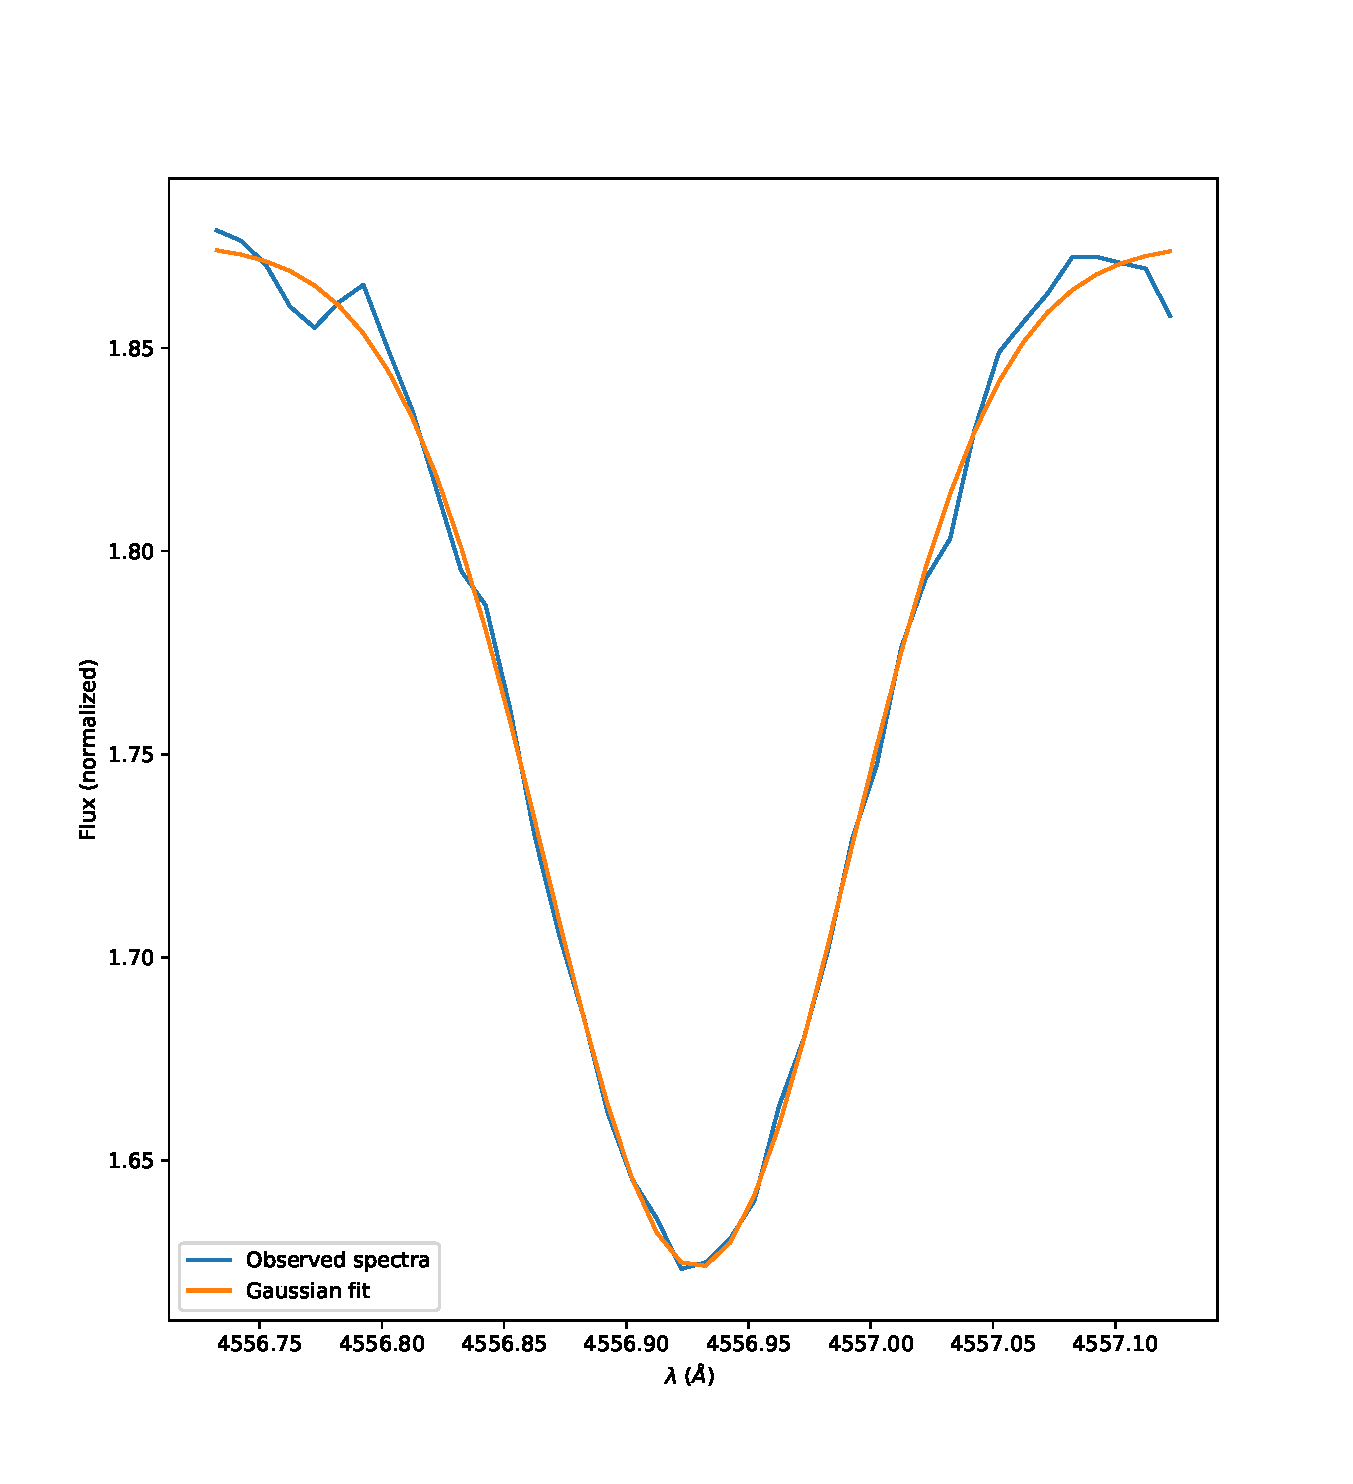
\includegraphics[width=\linewidth]{line_fit1.pdf}
  \caption{Gaussian fit to spectral line}
  \label{fig:line_fit}
\end{figure}


\subsection{Temperature estimation}
\label{sec:temp_estimation}

With efficiency in mind, we start by estimating the effective temperature of our
spectra, as this allows us to limit the range of spectra to lookup in the
database greatly. We achieve this by calculating the equivalent width of lines
of two multiplets of sufficiently different excitation energy and plotting
$log \left(  W / \lambda \right)$ by $\log \left( g f \lambda \right)$. From the
relation (\cite{monteiro_sebenta_2019}) 

\begin{equation}
  \label{eq:log_W_relation}
  \log \left( \frac{W_\lambda}{\lambda} \right) = \alpha  + \log \left( \lambda f_i g_i \right) - \frac{5040}{T_{\text{exc}}} \chi_i
\end{equation}

with $\log \left( \lambda f_i g_i \right)$ and $\chi_i$ know for each multiplet
(\cite{tsantaki_deriving_2013}), and $\alpha$ a constant, we may denote the average distance between
linear fits (for which equation \ref{eq:log_W_relation} is common) as $\Delta$ and obtain

\begin{equation}
  \label{eq:T_exc}
  T_{\text{exc}} = \frac{| 5040 \left( \chi_2 - \chi_1 |\right)}{\Delta}
\end{equation}


Using known equivalent widths for the sun's lines (Figure \ref{fig:temp_estimation_sun})
we get $T = 5769$ K directly from equation \ref{eq:T_exc}.

\begin{figure}
  \centering
  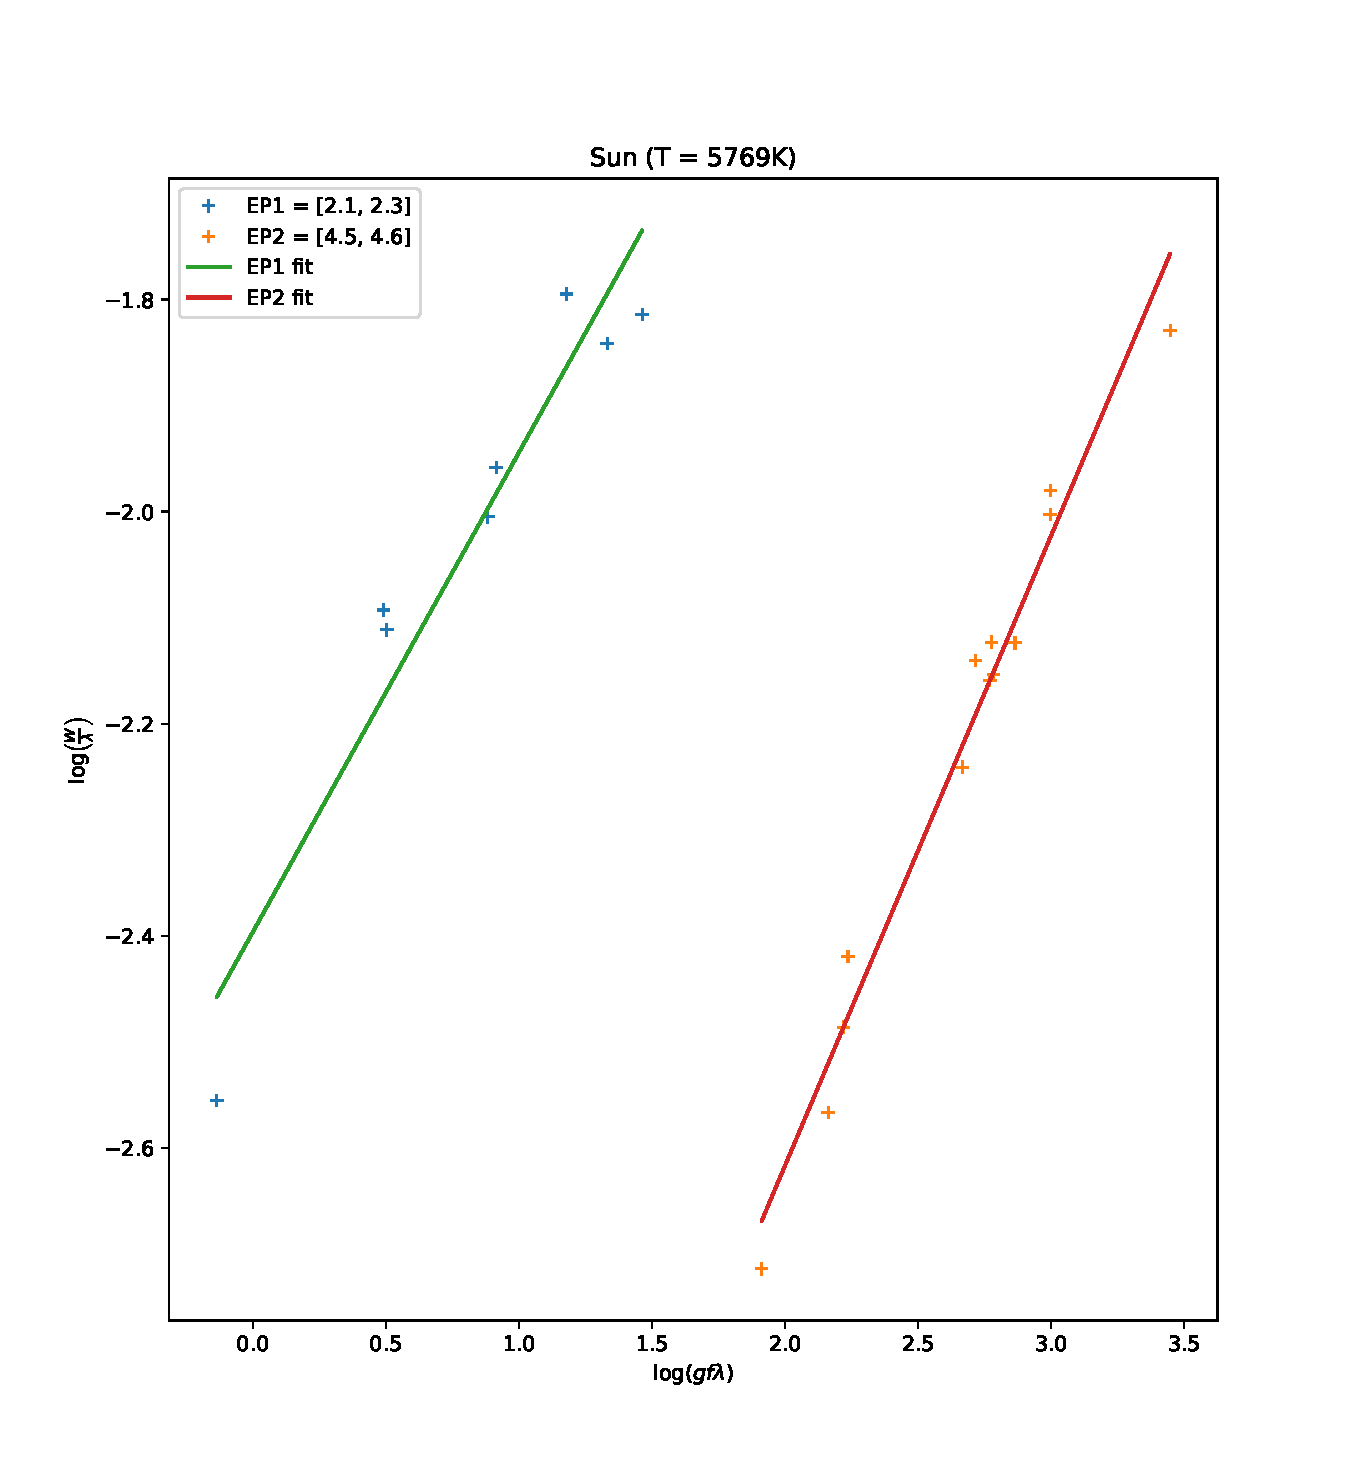
\includegraphics[width=\linewidth]{temperature_estimation_sun.pdf}
  \caption{Sun's temperature estimation}
  \label{fig:temp_estimation_sun}
\end{figure}

\subsection{Synthetic spectra database lookup and comparison}
\label{sec:database_lookup}

Setting an uncertainty interval on the temperature $\Delta T$  (in our case,
$\Delta T$ = 400K), one may now compare the observed spectra with synthetic
spectra (in \cite{laverny_ambre_2012}) with temperatures in the range $T\in [T - \Delta T, T + \Delta T]$.

This comparison proceeds once again by calculating the equivalent width of known
lines of both spectra. We may then plot $W_\text{synt}$ by $W_\text{obs}$ and
determine the best synthetic spectra by determining the one
corresponding to a linear fit of slope closest to unity. \footnote{Alternatively, a least squares
  comparison may be used. The reasons for not using this method will be
  clarified later. They may nevertheless be reduced to equivalent methods,
  depending on the choice of lines. Due to the efficiency of computational
  fitting methods, there is no significant slowdown.}


\subsection{Synthetic spectra processing}

With the best fitting spectra found, one need only process it before the comparison
with the observed spectra. This consists of:

\begin{enumerate}
\item applying the experimental profile of
  the instrument of measurement used, by means of a convolution of the spectra
  with a Gaussian determined by the experimental parameters as in equation
  \ref{eq:exp_profile_params} (\cite{monteiro_sebenta_2019}).

  \begin{equation}
    \label{eq:exp_profile_params}
    \sigma = \frac{<\lambda>}{R \sqrt{8 \ln (2)}}
  \end{equation}

  being $\sigma$ the standard deviation of the Gaussian function and $R$ the
  resolution of the instrument ($R \approx 50000$ for HARPS used in \cite{tsantaki_deriving_2013}).
\item estimating the rotational velocity of the star $v \sin I$ by Fourier analysis
  of the spectra and averaging the minima its FFT (see figure
  \ref{fig:line_fft}) over given lines and estimating $v \sin I$ by equation 

  \begin{equation}
    \label{eq:vsinI}
    v \sin I = \frac{\Delta \lambda_M}{\lambda_0} c
  \end{equation}

  where $c$ is the speed of light, $\lambda_0$ the central wavelength of the
  line, and $\Delta \lambda_M$ obtained by comparison with the values for the
  Sun, assuming linear limb darkening. \cite{monteiro_sebenta_2019}

  \begin{figure}[h]
    \centering
    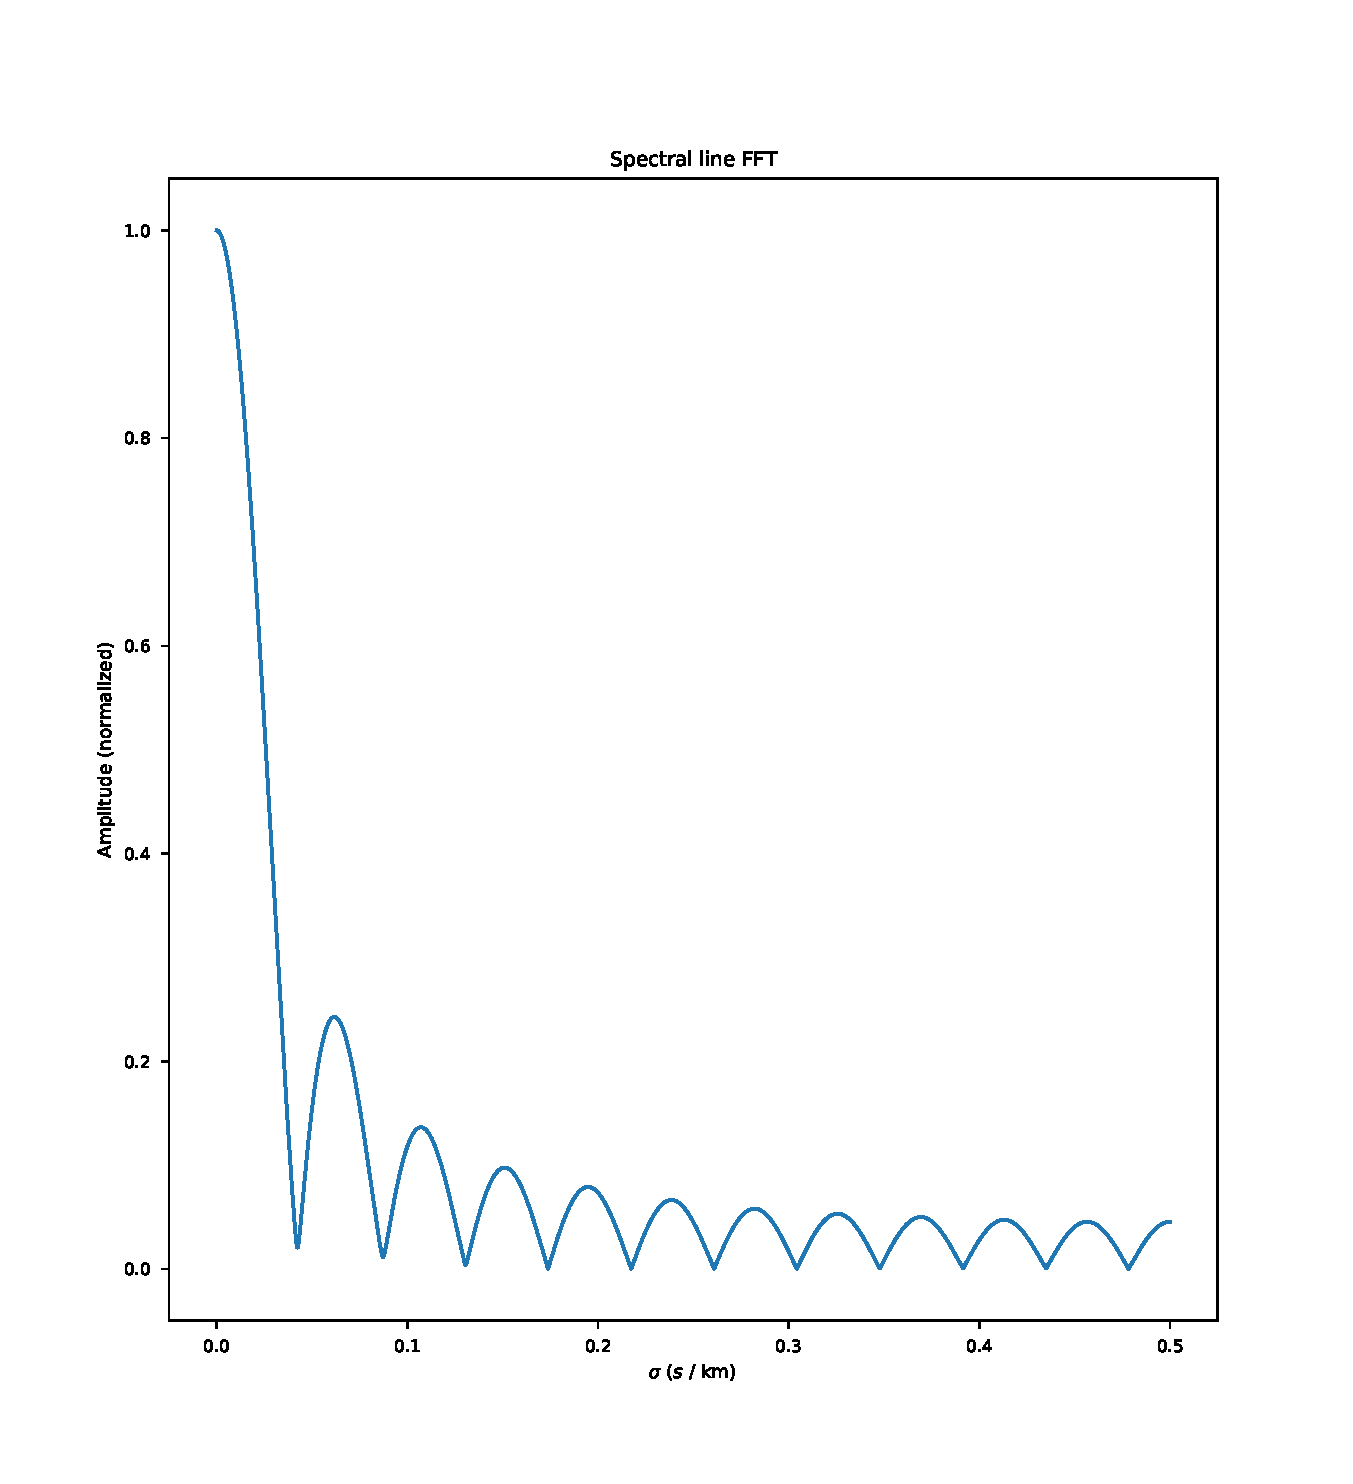
\includegraphics[width=\linewidth]{line_fft.pdf}
    \caption{Spectral line Fourier Transform}
    \label{fig:line_fft}
  \end{figure}
 
\item if rotational velocity is significant, applying a rotational profile to the
  spectra by convolution with a function of the type in equation \ref{eq:rot_profile}
  (illustrated in figure \ref{fig:rot_profile}). \footnote{For our analysis, we
    estimate $\epsilon$ by using it's value for the Sun.}
  \begin{equation}
    \label{eq:rot_profile}
    G_{\epsilon}\left(\lambda-\lambda_{0}\right)=\frac{2(1-\epsilon)\left(1-\left(\frac{\lambda-\lambda_{0}}{\Delta \lambda_{M}}\right)^{2}\right)^{1 / 2}+\frac{\pi \epsilon}{2}\left(1-\left(\frac{\lambda-\lambda_{0}}{\Delta \lambda_{M}}\right)^{2}\right)}{\pi \Delta \lambda_{M}(1-\epsilon / 3)}
  \end{equation}

  \begin{figure}[h]
    \centering
    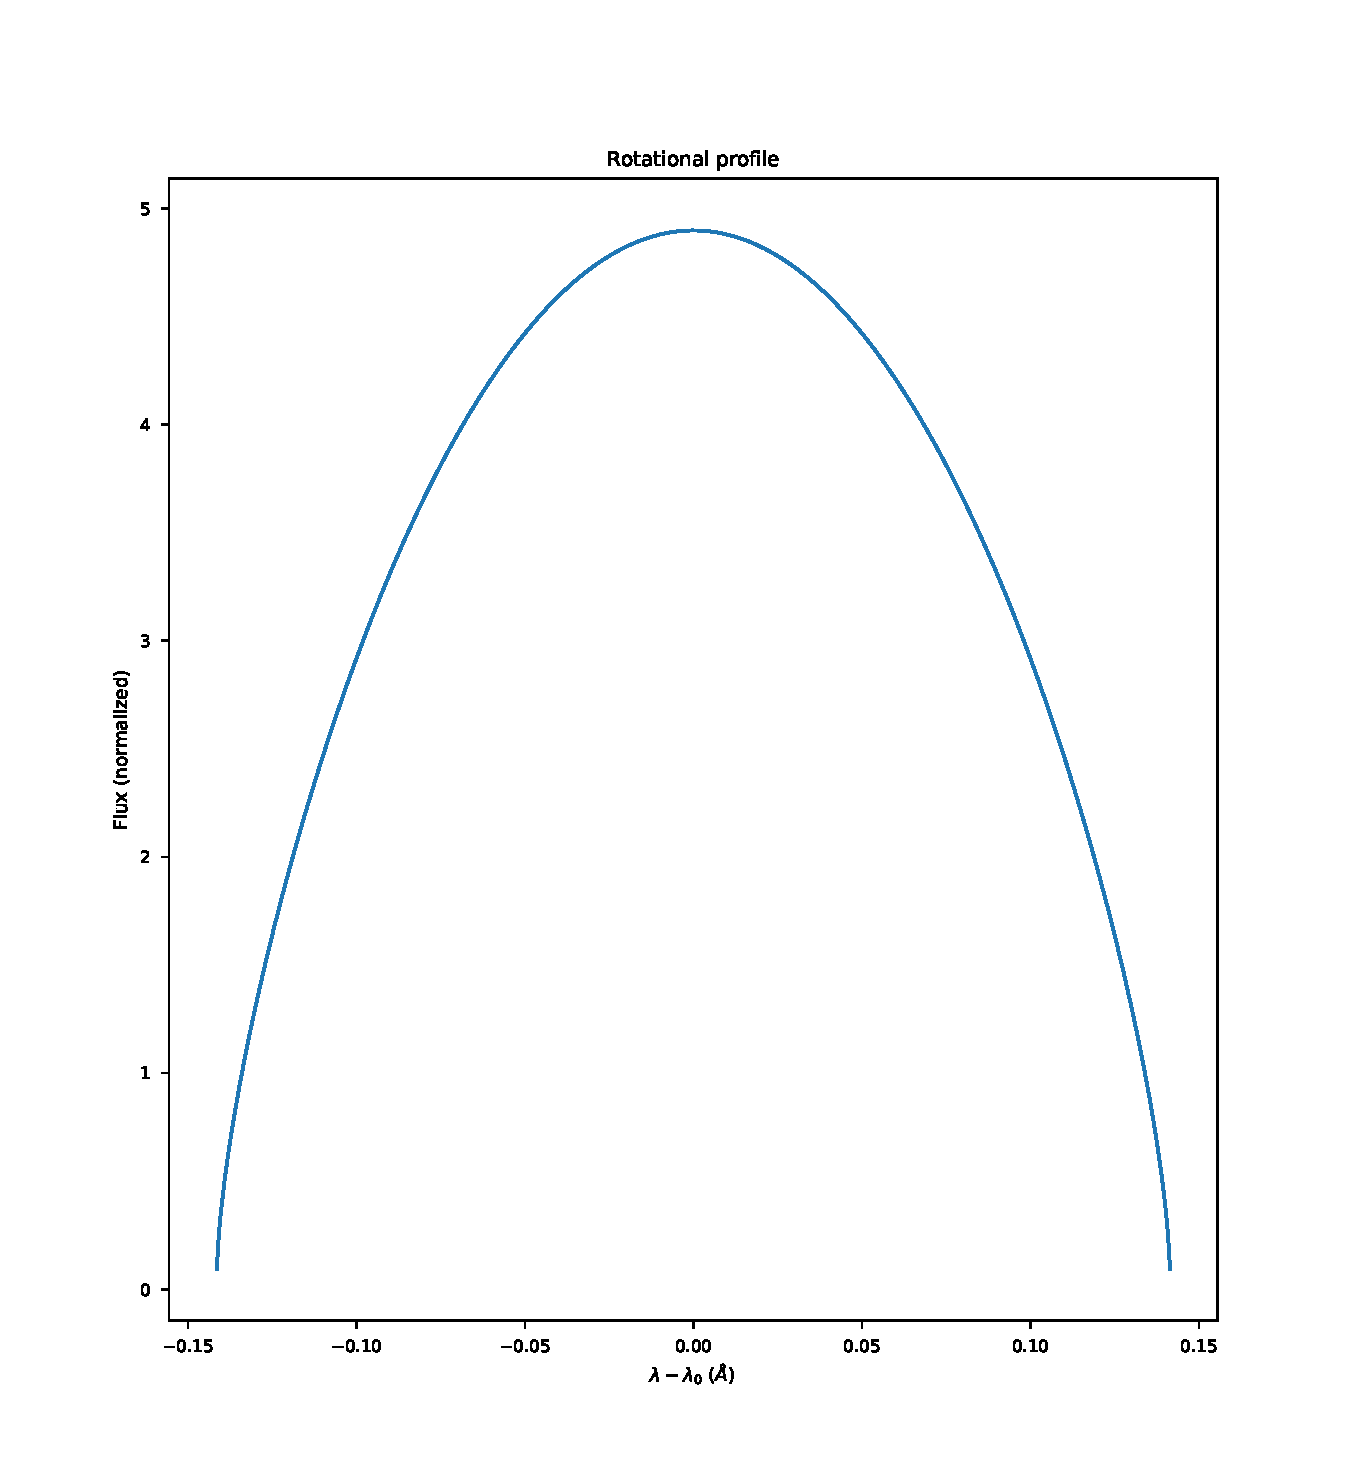
\includegraphics[width=\linewidth]{rot_profile.pdf}
    \caption{Rotational profile}
    \label{fig:rot_profile}
  \end{figure}
  
\item interpolating the synthetic spectra with observed data
  for ease of posterior analysis. 
\end{enumerate}


\section{Fitting pathologies}

In some spectra we noted some pathological behavior and conformed our method
to avoid it as systematically and consistently as possible. What follows is the
analysis of such cases and discussion of the workarounds used.

\subsection{Fitting lines - $k$ parameter}
\label{sec:k}

While the fitting of lines in observed spectra with fixed $k$ works well, it
becomes a problem when calculating equivalent widths of lines in synthetic
spectra. In these, multiple lines may get mixed together resulting in the
broadening and partial overlapping, as seen in figure \ref{fig:bad_synth_lines}.

\begin{figure}[h]
  \subfigure{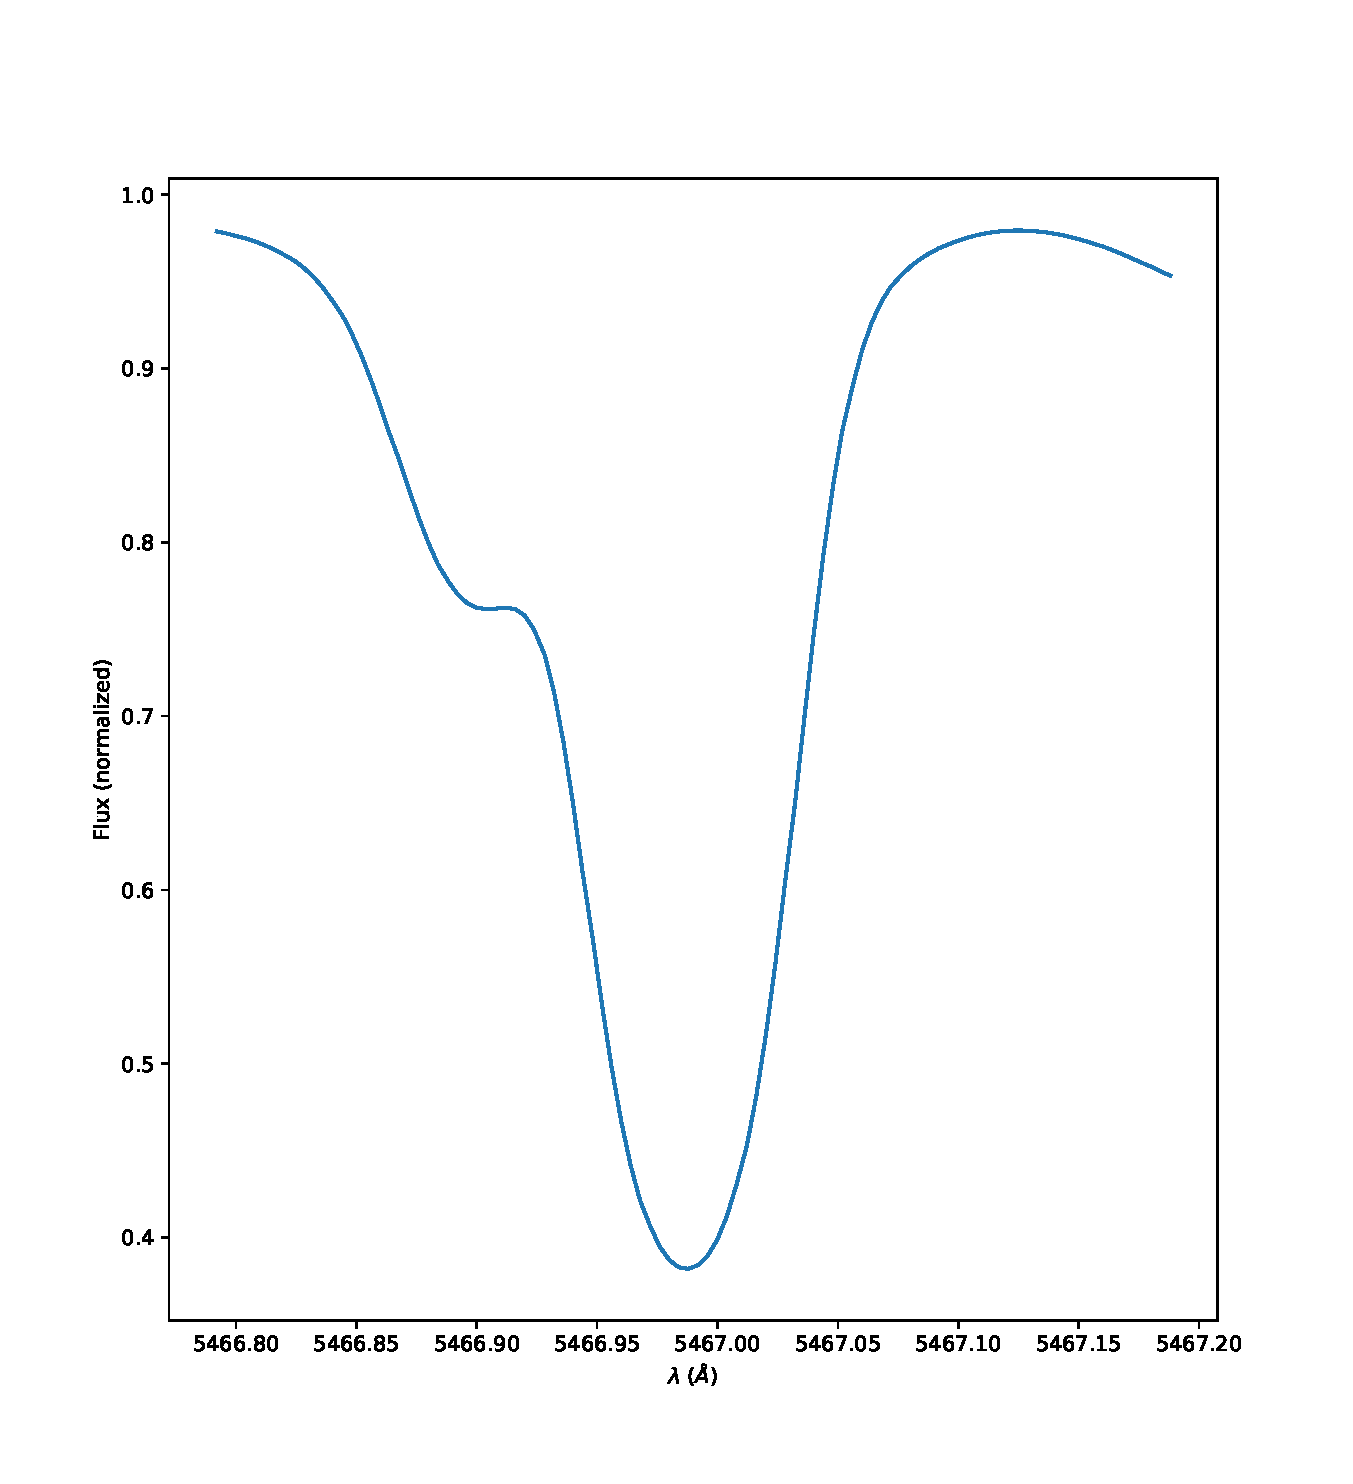
\includegraphics[width=.49\linewidth]{bad_synth_overlap.pdf}}
  \subfigure{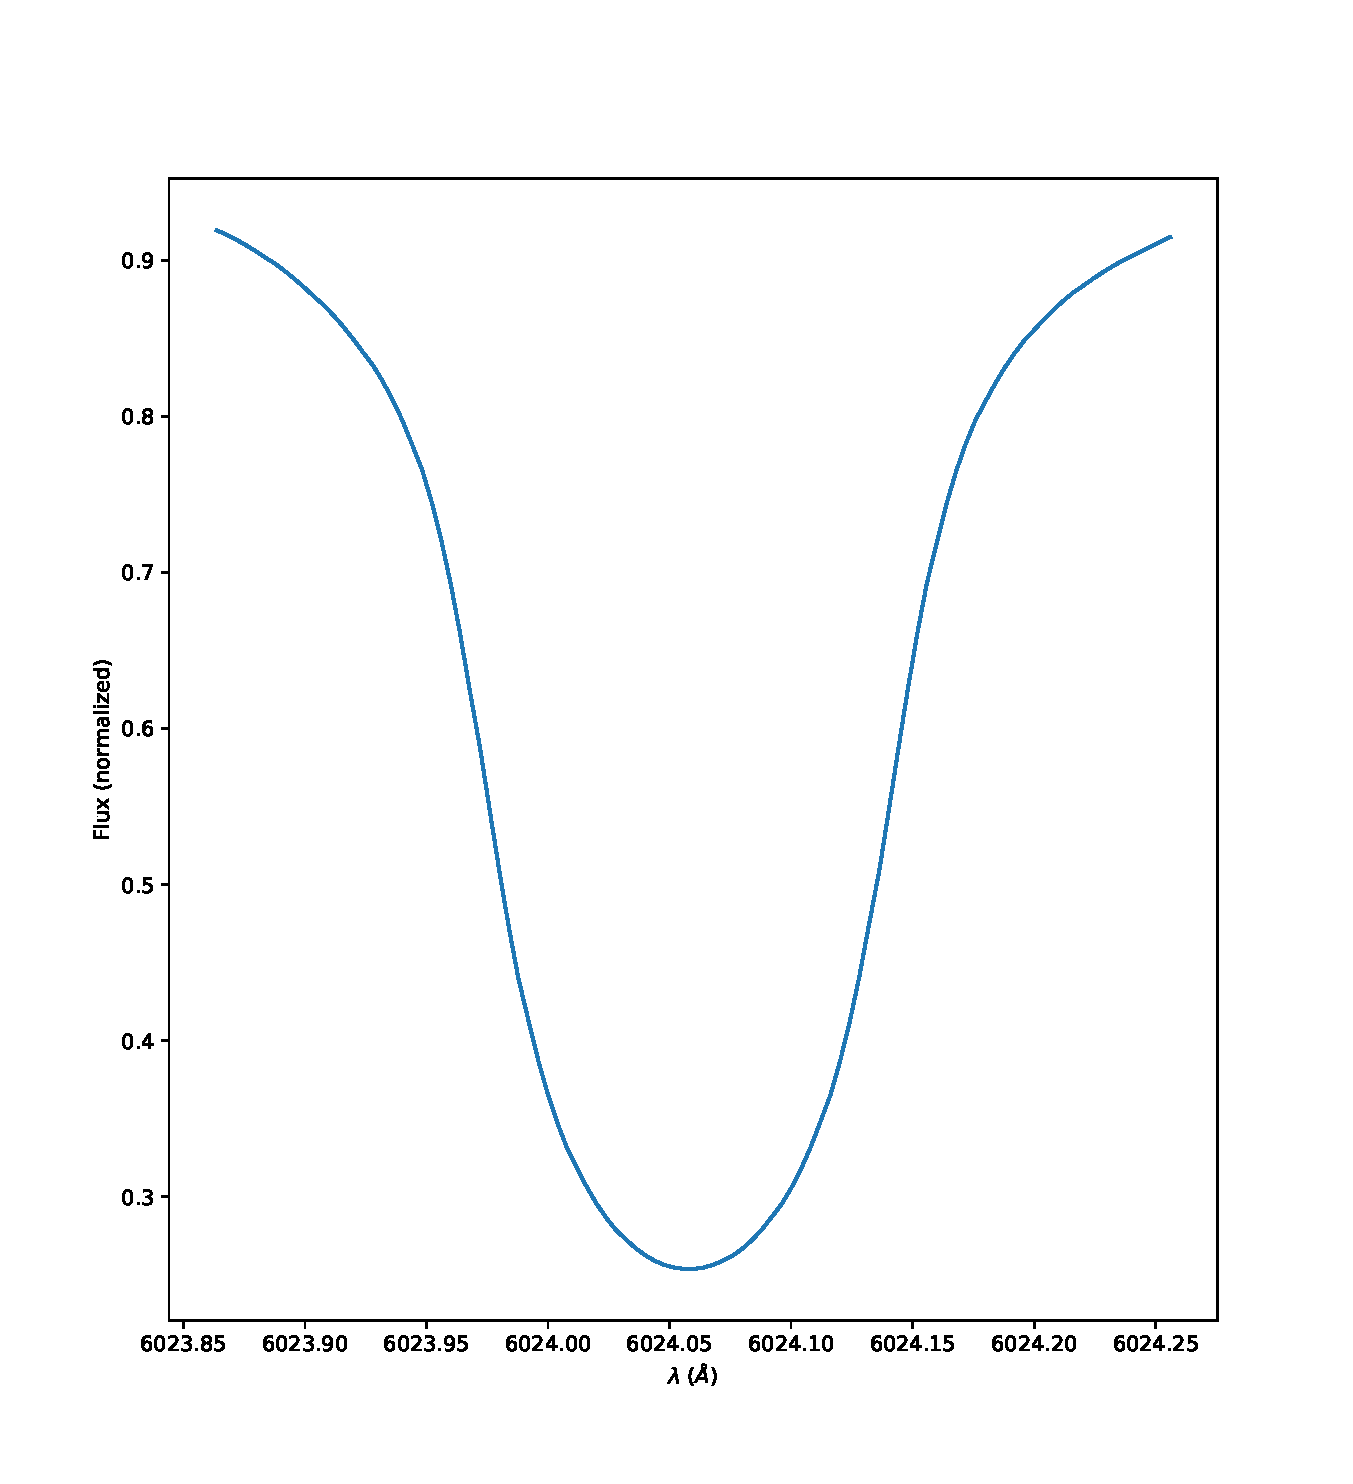
\includegraphics[width=.49\linewidth]{bad_synth_broadening.pdf}}
  \caption{Behavior of synthetic spectral lines}
  \label{fig:bad_synth_lines}
\end{figure}

Here, as efficiency is key, we take advantage of the well-behaved nature of the
synthetic spectra and evaluate a step difference function (calculating average difference
between points) evaluate the first and second derivative of the function. Our method, however,
  scales with $\mathcal{O}(n)$.} that allows us to limit a line to its
surrounding maxima, henceforth using the limited line to calculate equivalent
widths. The parameter $k$ in equation \ref{eq:W_estimation} is therefore automatically determined for these
spectra.

The adaptation of this method to the observed spectra is non-trivial because of experimental noise.

\subsection{Variable initial conditions in Gaussian fits}

The aforementioned behavior of synthetic spectra (or other conditions such as
high rotational velocity or turbulence) may induce problems while trying to employ Gaussian
fits, with significant line width variation. We handle this by varying the
proposed initial conditions for the fit and comparing residuals until we get a
good fit.

With effect, this implementation makes it possible to automatically determine
the quality of a fit. If no parameters provide a good fit, a line may not
behave as a Gaussian (as mentioned in section \ref{sec:k}), and can be safely ignored.

\subsection{Continuum estimation}
\label{sec:continuum_estimation}

The main difficulty of our method lies with calculating an accurate estimation of
the continuum of the spectra for each line. In general, observed spectra may not be
normalized and, because of the characteristics of the instrumentation used, have
a different continuum level for different wavelengths.

One can chose from many methods to approach this problem. In the following we discuss the
advantages and disadvantages of some of the methods attempted. Additional
possible solution are discussed in section \ref{sec:improvements}. \footnote{This
  step in our algorithm is purposely left as modular and independent from the
  rest as possible so different methods may be tried with minimal
  reformulation of the program.}

\subsubsection{Normalizion with additive Gaussian parameter}
\label{sec:norm1}

If we are adjusting a Gaussian of the form $a \exp \left[ \frac{(x-b)^2}{2c^2} \right] +
d$ to the line, we may take the additive parameter $d$ as the continuum line and
in this manner normalize each line.

This method is vulnerable to the cases where lines are influenced by its
neighbors (figure \ref{fig:additive_parameter}).

\begin{figure}[h]
  \centering
  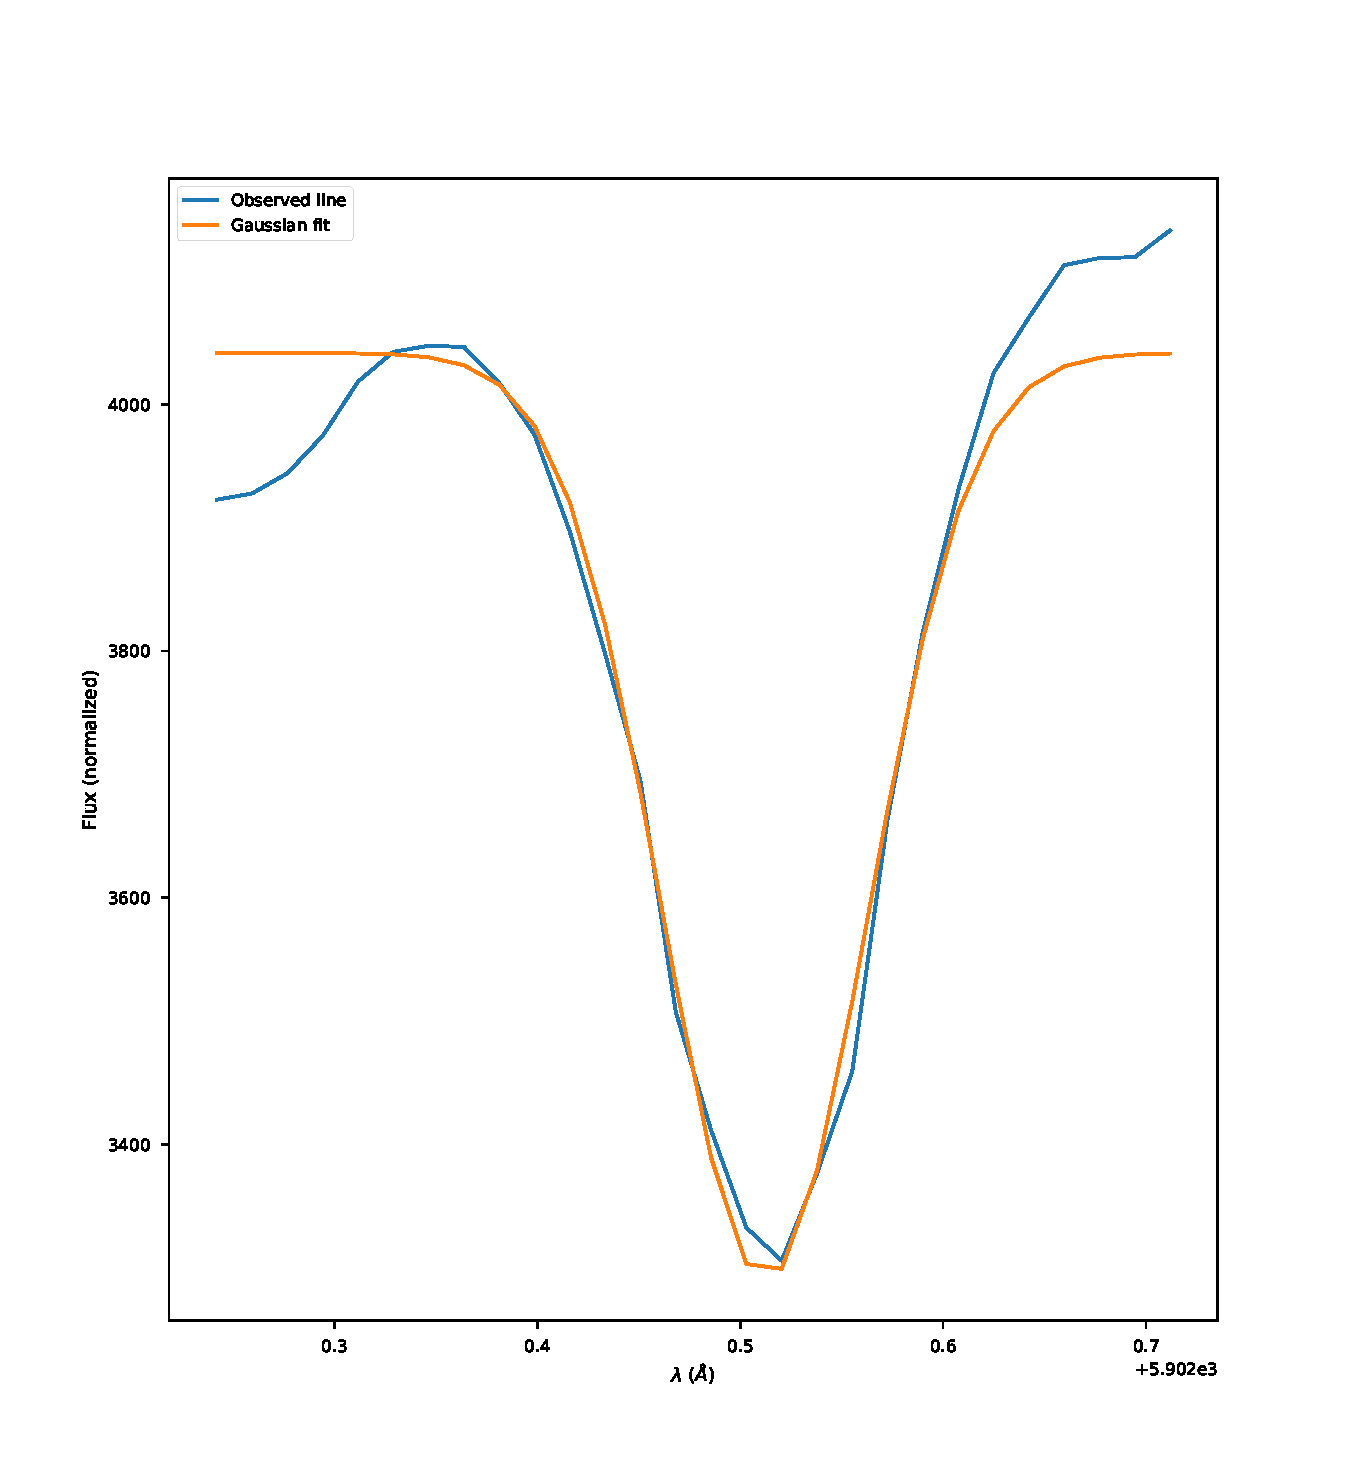
\includegraphics[width=\linewidth]{normalization_with_d.pdf}
  \caption{Pathological case for normalization with additive parameter}
  \label{fig:additive_parameter}
\end{figure}

However, some of this cases may get caught automatically if we refine a
tolerance in the estimated quality of the fit sufficiently well.

\subsubsection{Normalization by limit estimation}
\label{sec:norm2}

An alternative approach may be to calculate the continuum by averaging the
values of the spectra at the line extrema, normalizing the spectra locally
before fitting.

This shifts the source of uncertainty in the calculation from the quality of the
fit to the estimation of the extrema. If the width of the lines is not predictable
along the wavelength range limiting the line properly may be problematic.

\subsection{Multiplet selection}
\label{sec:multiplet_selection}

The choice of multiplet used for comparison in temperature estimation (section
\ref{sec:temp_estimation}) need carefully adhere to the conditions:

\begin{enumerate}
\item Both multiplets may be restricted to a small excitation energy range EP1 and EP2.
\item EP1 and EP2 be sufficiently distinct from each other. 
\item Lines to be considered in a given multiplet should have similar wavelength.
\item Energy ranges are associated with lines of comparable equivalent widths,
  so as to enable the computation of average distance between them.
\end{enumerate}

Even under these conditions, better results are obtained from multiplets corresponding
to growth curves of similar slope, as seen in figure
\ref{fig:temp_estimation_sun}. For keeping under these orientations, a casuistic
verification may be needed for optimal results.


\subsection{Linear fit method for determining best synthetic spectra}

As referenced in section \ref{sec:database_lookup}, the linear fitting method
used to compare spectra is generally equivalent to a least squares algorithm.
However, that is only true if we are able to compute $W$ of every synthetic
line.

In our algorithm, the number of fitted lines may vary from spectra to spectra.
As such, employ a linear fitting method, evaluating the difference from unity slope in
the plot $W_\text{synt}$ vs $W_\text{obs}$, because it is independent of the number of lines fitted.

\section{Applications}

\subsection{Iota Horologii (HD 17051)}
\label{sec:star1}

The application of our algorithm to HD 17051, a star of low rotational velocity,
is immediate, as the observed spectrum used was previously normalized.

\begin{figure}[h]
  \centering
  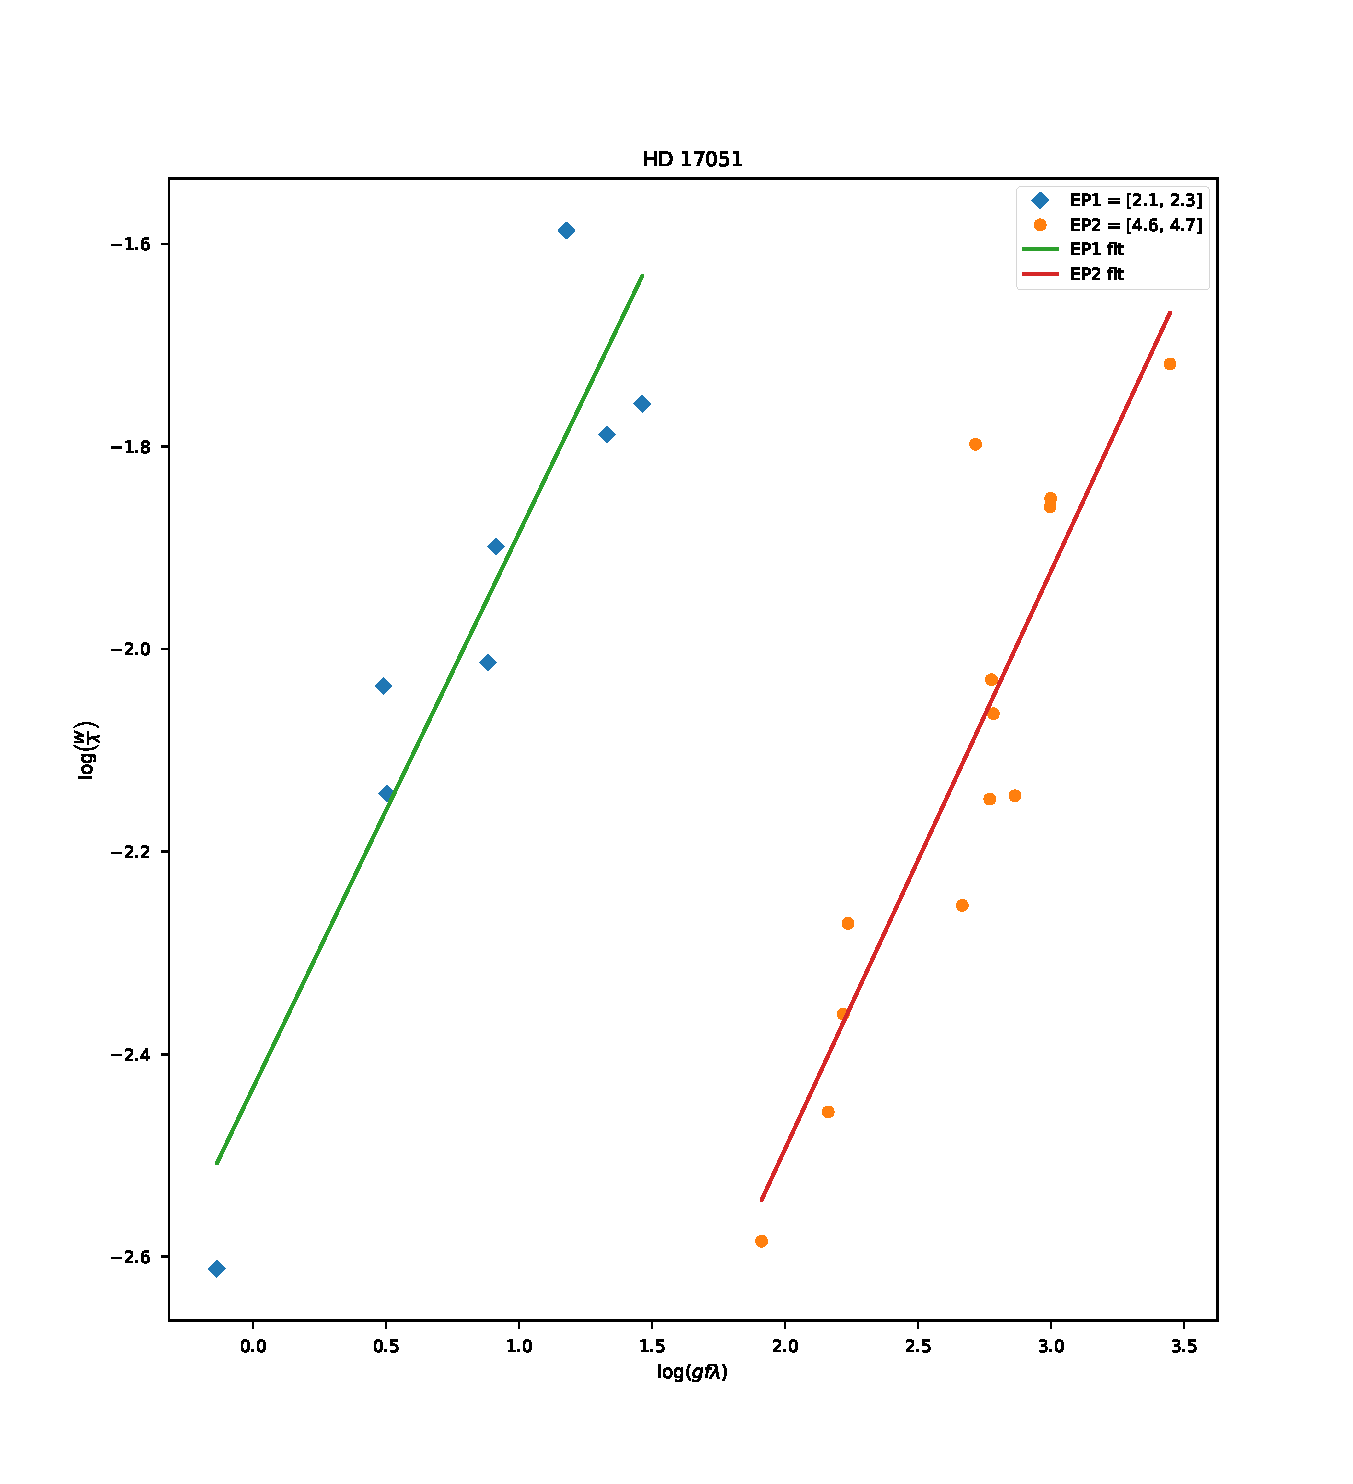
\includegraphics[width=\linewidth]{temperature_estimation_star1.pdf}
  \caption{HD 17051 - $T_\text{eff}$ estimation}
  \label{fig:star1_temp_estimate}
\end{figure}

We get an estimate of the effective temperature of $T_\text{eff} = 6085K$, from
the growth curves in figure \ref{fig:star1_temp_estimate}. \footnote{The
  multiplets used do not strictly obey the conditions of listed in section
  \ref{sec:multiplet_selection}, in the sense that we use a wide range of
  wavelengths. This was used because using strictly two simple multiplets as
  described would provide a small number of equivalent widths to compare.
  This is a consequence of the size of our line database. Special attention was
  used to guarantee that the growth curves behave as expected.}

For this star, all observed lines could be fitted with our algorithm, which
found the best fit in our database (\cite{laverny_ambre_2012}) listed in table
\ref{tab:star1_params}, compared with measured parameters from \cite{suarez-andres_c/o_2018}.

\begin{figure}[h]
  \centering
  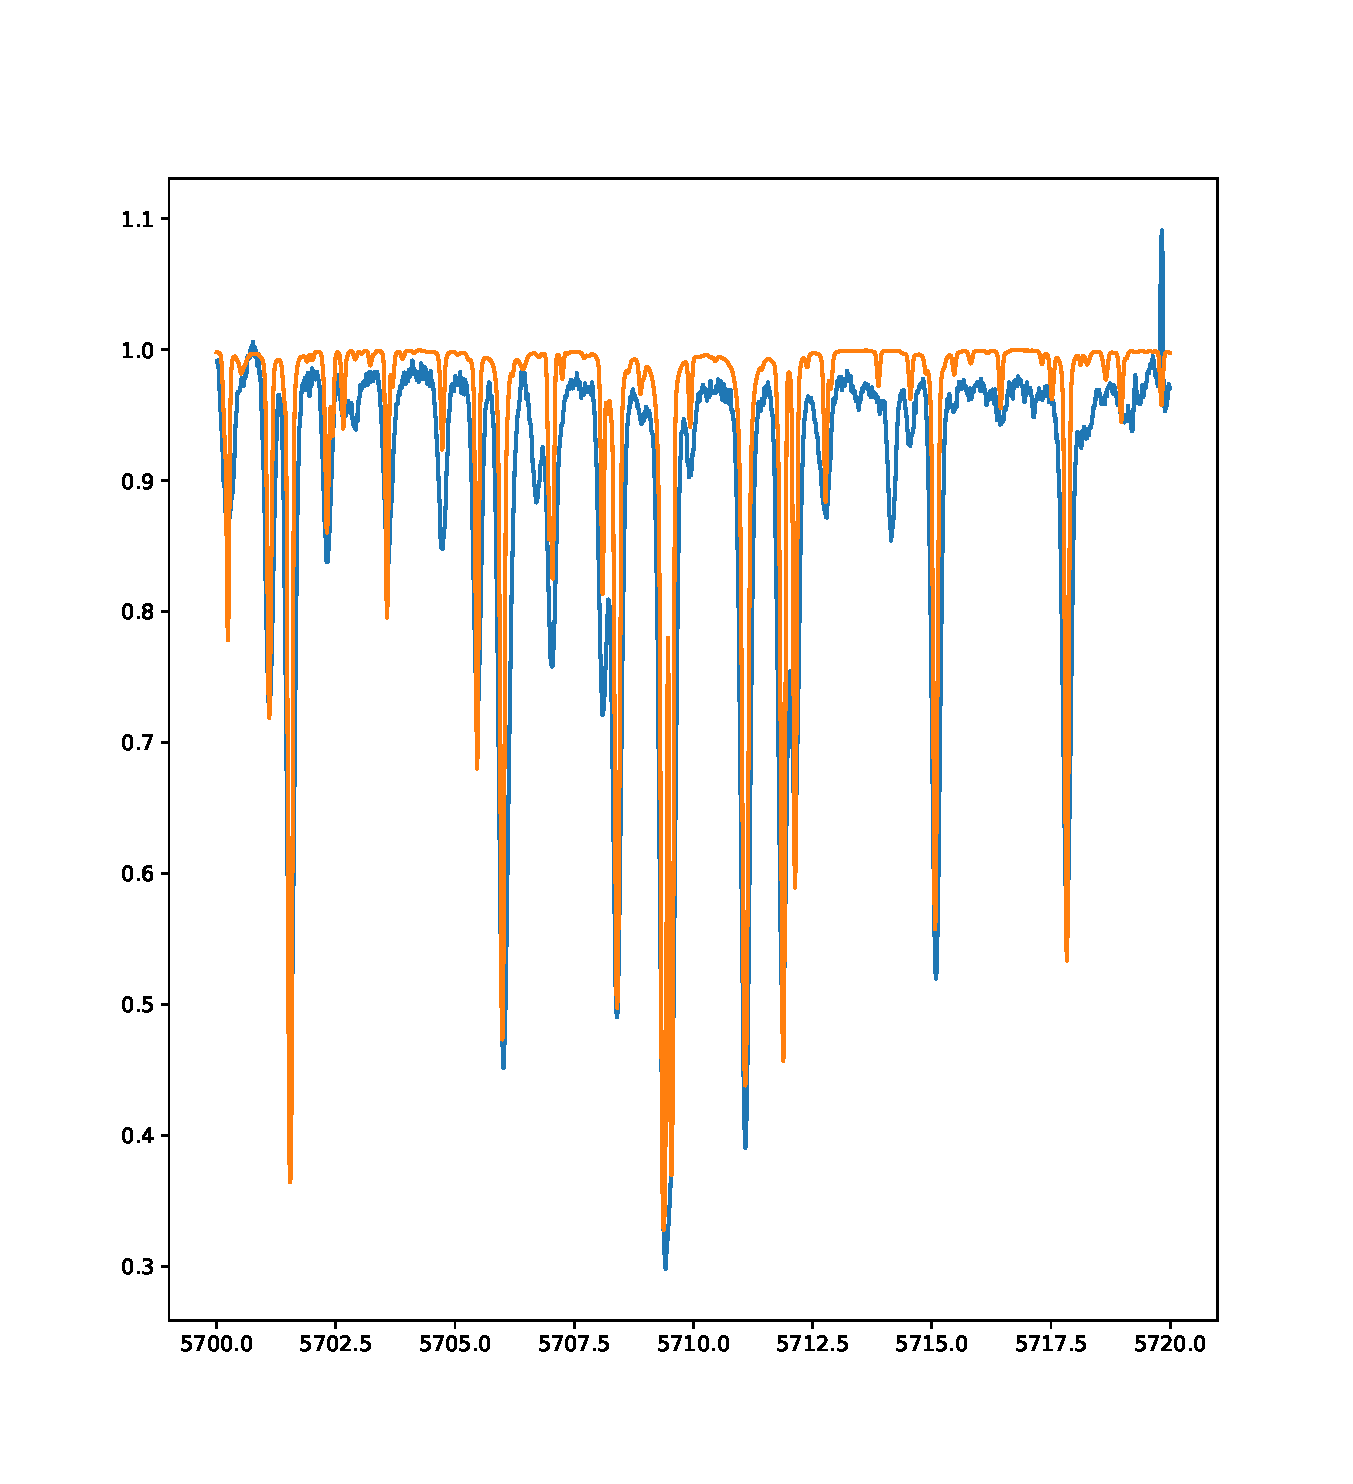
\includegraphics[width=\linewidth]{best_fit_star1.pdf}
  \caption{HD 17051 - Best fitting spectrum}
  \label{fig:star1_best_fit}
\end{figure}


\begin{table}[h]
  \label{tab:star1_params}
  \centering
  \begin{tabular}{c  c  c}
    Parameters & Algorithm & Literature \\
    \midrule
    $T_\text{eff}$ (K) & 6000 & 6122 \\
    $\log g$  & 4.5 & 4.37 \\
    $Z$ & 0.25 & 0.17 \\
    $a$ & 0.0 &  ---
  \end{tabular}
  \caption{HD 17051 - stellar parameters}
\end{table}

The chosen spectra may also be visually compared (see figure
\ref{fig:star1_best_fit}). It is clear from visual comparison that not all
lines are similar between the spectra. This, of course, is consequence of the
coarse parameter space of the database, and of only using some lines for comparison.


\subsection{24 G. Virginis (HD 104304)}
\label{sec:star2}

We now treat the case of HD 104304, an example of cooler object, with
significant rotational velocity.

Like before we estimate the temperature (figure \ref{fig:star2}) getting $T_\text{eff} =
5415 K$ and the algorithm chooses the spectrum with parameters from table
\ref{tab:star2_params} (comparison with \cite{aguilera-gomez_lithium_2018}).

\begin{figure}
  \subfigure{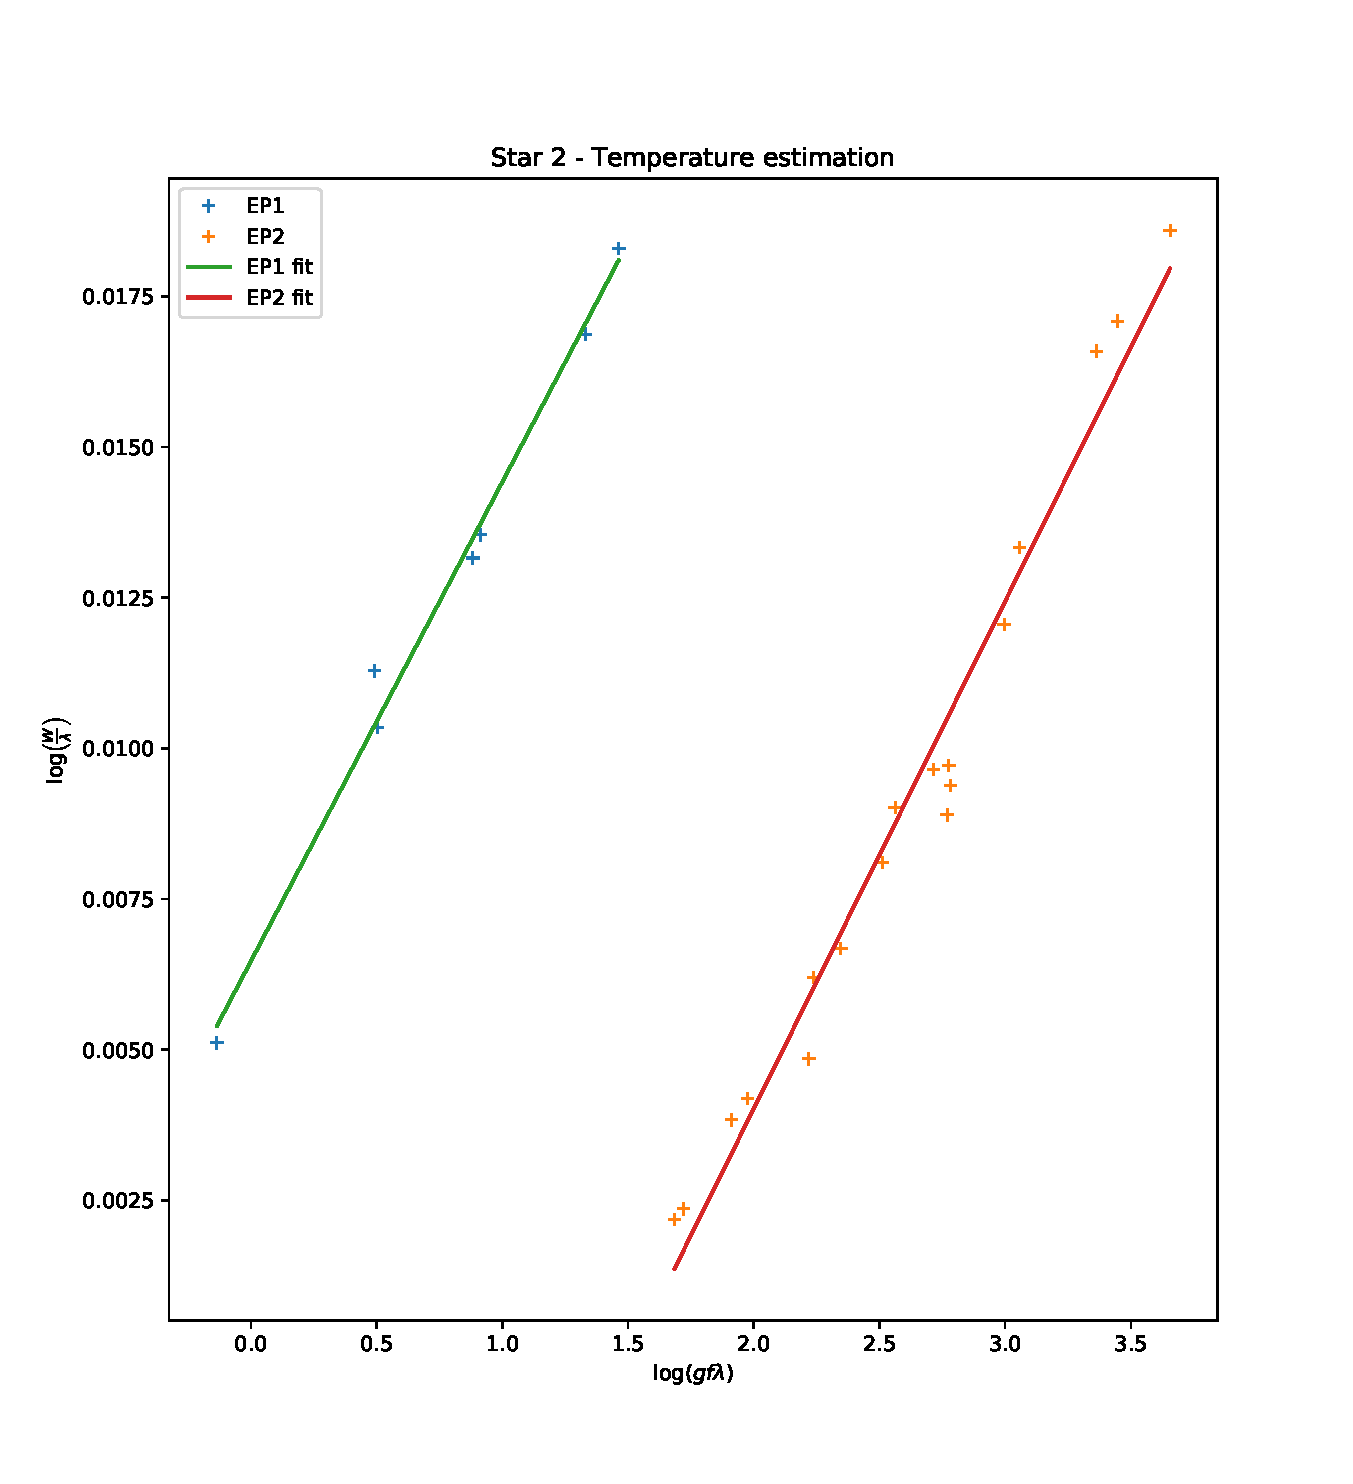
\includegraphics[width=.49\linewidth]{temperature_estimation_star2.pdf}}
  \subfigure{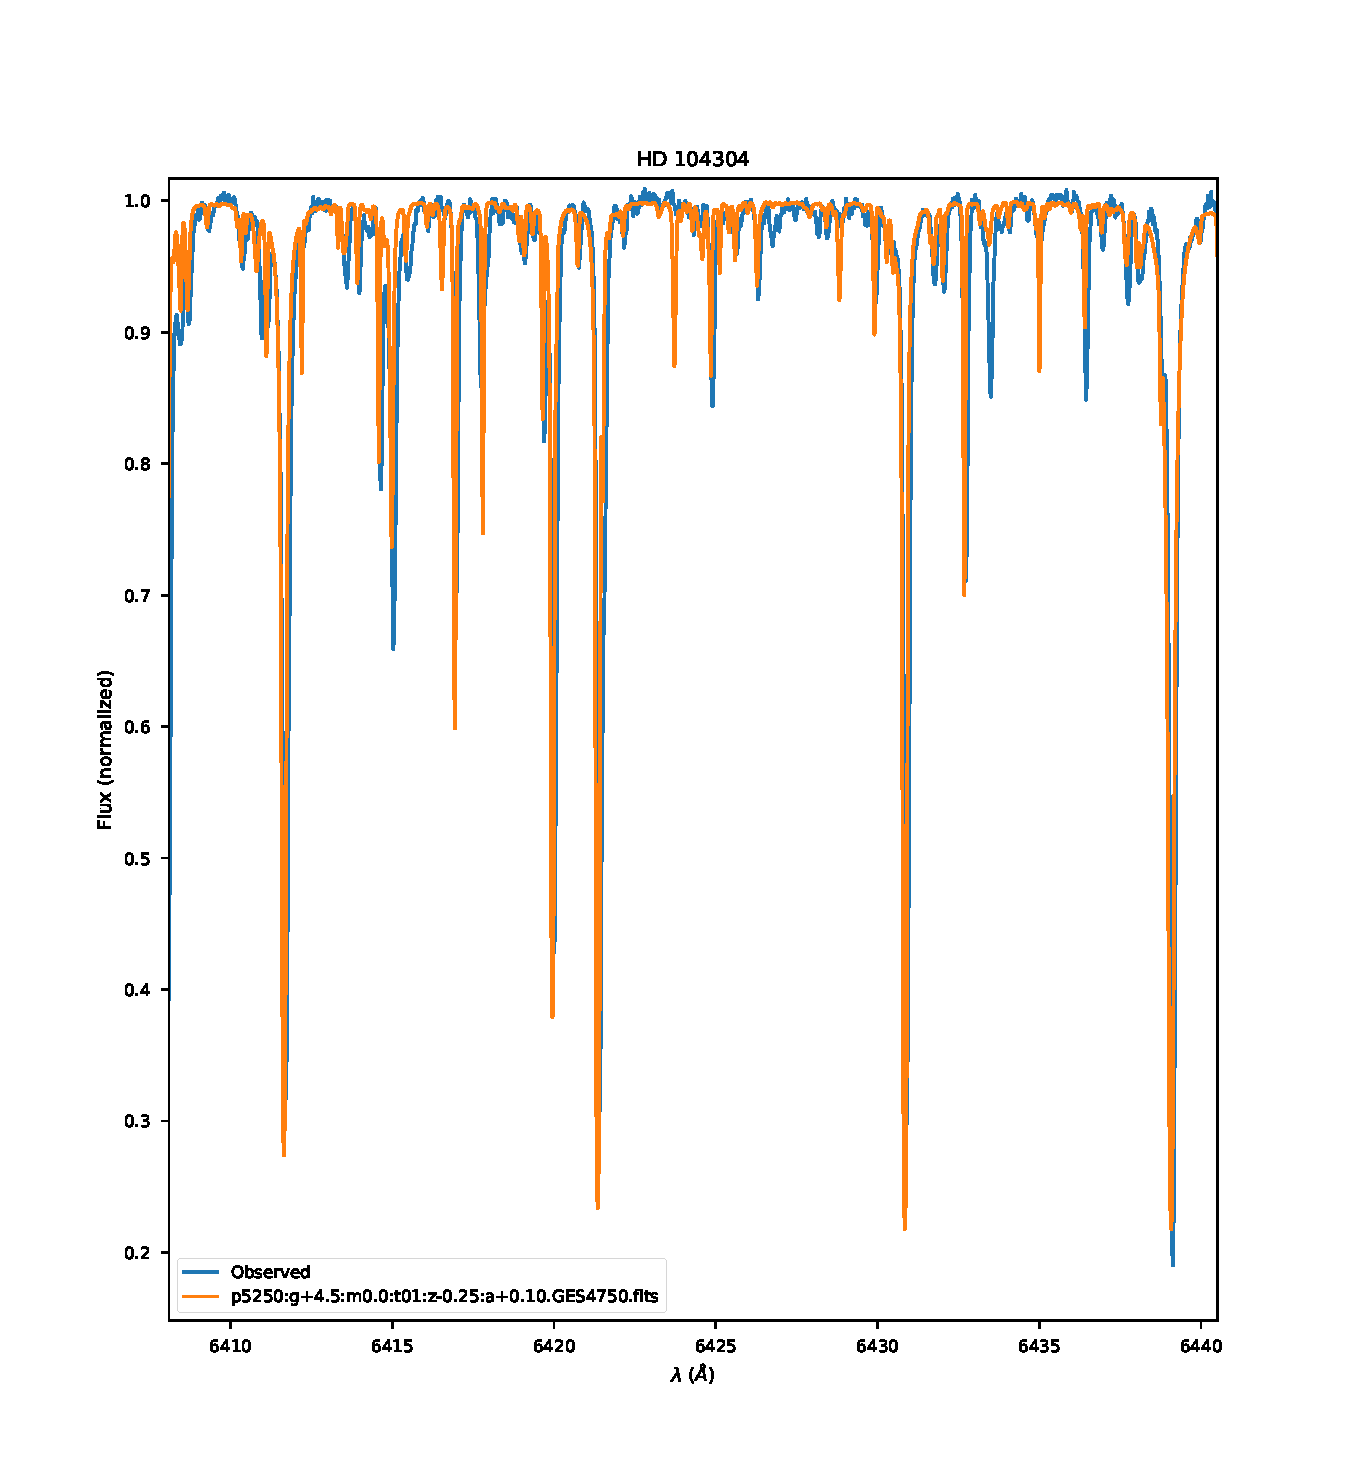
\includegraphics[width=.49\linewidth]{best_fit_star2.pdf}}
  \caption{HD 104304 temperature estimation and spectra comparison}
  \label{fig:star2}
\end{figure}

\begin{table}
  \label{tab:star2_params}
  \centering
  \begin{tabular}{c  c  c}
    Parameters & Algorithm & Literature \\
    \midrule
    $T_\text{eff}$ (K) & 5250 & 5506 \\
    $\log g$  & 4.5 & 4.42 \\
    $Z$ & -0.25 & 0.31 \\
    $a$ & 0.10 &  --- \\
    $v \sin I$ (km$s^{-1}$) & 6.5 & 5.2
  \end{tabular}
  \caption{HD 104304 - stellar parameters}
\end{table}

The observed spectrum used in this case was not previously normalized, so we see
a more significant error from the continuum estimation. The broadening of lines
caused by the significant rotational velocity also causes this behavior. Our
results are therefore a worse estimation of stellar parameters.

\section{Possible improvements}
\label{sec:improvements}

The greatest improvement to this project would come from a refinement of the
method used to estimate the local continuum of observed spectra.

One way to go about doing this would be to consider a region around each line,
determine the approximate location of all the lines (by computing the second and
third derivatives of the spectra, for example), and employing multiple Gaussian
fits to the region. This complete information about the line and its neighbors
would allow for a much more precise measurement of the continuum value locally.

This method, however, due to the need to estimate line locations (or indirectly,
spectra derivatives) is much more sensible to noise, so a noise reduction
algorithm would need to be implemented. For this reason, said approach lies
beyond the scope of our algorithm, but is used by projects such as ARES (\cite{sousa_ares_2015}).

Our results would also be improved by implementing a wider range of possible
functional fits for spectral lines, such as Lorentzian or Voigt profiles. Due to
the modular nature of the code, this would be a relatively straightforward implementation.

Application wise, better results would be an immediate consequence of more
extensive and parameterically dense line and spectra databases.

%-------------------------------------------------------------------
\section{Conclusions}

\begin{itemize}
\item An efficient algorithm was developed to determine stellar
  parameters such as temperature, $\log g$ and metallicity from spectrocospic
  analysis, by equivalent width comparison.
\item The implementation was detailed and different methods discussed.
\item Pathological cases were displayed and possible solutions and improvements were discussed.
\item An effective application of the algorithm was showed and consequent
  results discussed.
\end{itemize}

For more information on the code visit: \url{https://github.com/ruimpz/spectra}.

\begin{acknowledgements}
  This work was done under the orientation of professor Jorge Gameiro in the
  context of the curricular unit of Computational Astronomy.
\end{acknowledgements}

\bibliographystyle{aa}
\bibliography{spectra}

\end{document}